\documentclass{article}
\usepackage{CJKutf8}
\usepackage{graphicx}
\usepackage{color}
\begin{document}
\begin{CJK}{UTF8}{bkai}
\title{\Huge \color{blue} 聽歌辨識歌手  srs }
\author{第六組   李政憲 張哲郡 游登翔 劉彥麟 張友澤}
\maketitle
\begin{figure}[h]
\begin{center}
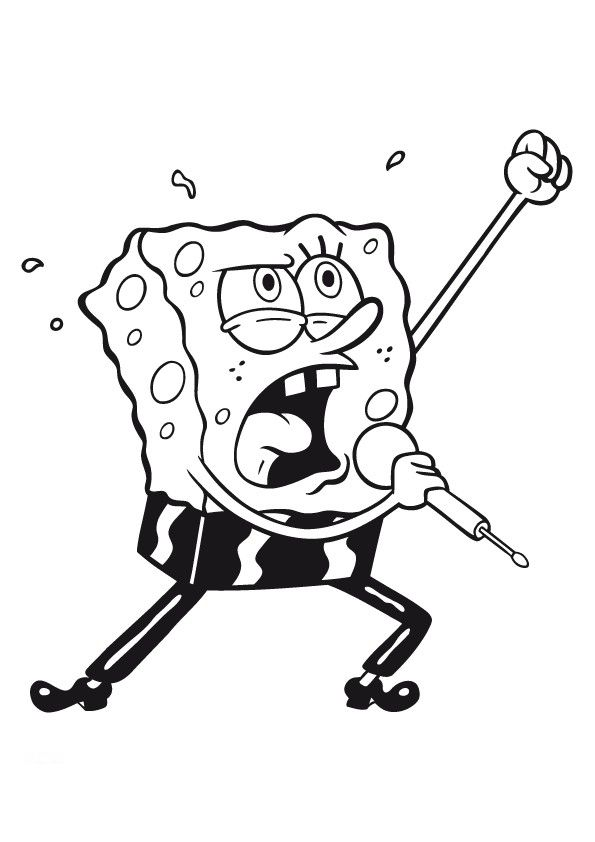
\includegraphics[width=8.5cm]{sing.jpg}
\end{center}
\label{fig:1}
\end{figure}
\newpage
\section{\huge \bf \color{blue}  introduction\\}

\subsection{\Large Purpose\\}
\large 做出一個只要輸入進去一首歌的音檔 就能判別出唱的歌手是誰的project
\subsection{\Large Intended Audience and Reading Suggestions\\}
\large intended Audience : 想要查詢自已聽到的歌是誰唱的的user \\\\
閱讀建議:對使用者而言要多注意"External interface"的部分\\
並且需要具備一定程式知識
\subsection{Project Scope\\}
這是個獨立的project, 
其目的為使user能辨識出聽到的歌是來自於哪位歌手

\newpage


\section{\huge\bf \color{blue}  Overall Description\\}

\subsection{\Large Product Perspective\\}
 \large 這個project利用很多首歌訓練出了各種歌手的特徵值 再利用這些特徵值辨別出我們輸入進去的是哪位歌手\\\\\\\\
\subsection{\Large Product Functions}
\large 輸入進去歌曲的音檔 就能讓它判斷是我們給的歌手們(分類)中的哪位\\\\\\\\

\subsection{\Large User Classes and Characteristics\\}
  \Large 聽線上電台的人, 實況的觀眾等等想知道當下聽到的歌是誰的歌的user\\\\
\newpage
\subsection{\Large Operating Environment \\}
 \Large Operating system: Windows 10\\
platform:pycharm python3\\
音訊處理:ffmpeg

\subsection{\Large Design and Implementation Constraints\\}
   \Large 因為大部分的歌都會有伴奏 \\
有些甚至快大過歌手本身的歌聲,\\
所以實際再辨別時是有難度的\\
音檔轉換為頻譜圖可能會失真
\subsection{\Large  Assumptions and Dependencies\\}
  \Large  這份專案是先假設即使沒有去除掉背景音\\
 電腦仍然能透過train來辨別出該歌手的特徵\\
並順利辨識

\newpage

\section{\huge\bf  \color{blue} External Interface Requirements\\}
\subsection{\Large User Interfaces\\}
\begin{figure}[h]
\begin{center}
\includegraphics[width=15cm]{software.png}
\end{center}
\label{fig:1}
\end{figure}
\subsection{\Large Hardware Interfaces\\}
windows 10//
\newpage
\subsection{\Large Software Interfaces\\}
operating system:windows
pycharm\\
ffmpeg

\newpage



\section{\huge\bf \color{blue}  System Features }
\subsection{\Large Description and Priority }
	將數據分類好放入 “/dataset”\\
	將所有歌手的mp3檔進行資料前處理壓縮成.npy檔\\
	使用.npy檔進行model的學習\\
	透過學習成果分辨其他mp3檔的歌手\\


\subsection{\Large Stimulus/Response Sequences}
\begin{figure}[h]
\begin{center}
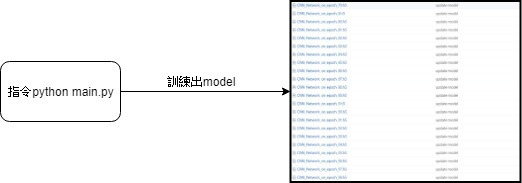
\includegraphics[width=8.5cm]{sti.jpg}
\newline
\newline
\newline
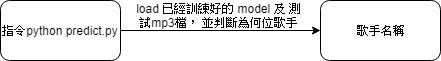
\includegraphics[width=8.5cm]{ss.jpg}
\end{center}
\label{fig:1}
\end{figure}

\subsection{ \Large Functional Requirements}
 REQ-1:新增歌手進入數據集


\section{\huge\bf  \color {blue}  Other Nonfunctional Requirements }
\subsection{ \Large Performance Requirements}
訓練歌手的mp3檔需200筆\\\\\\\\
\Huge\bf   Thank you for watching


\end{CJK}
\end{document}
